\documentclass[xetex,mathserif,serif,handout]{beamer}

\usepackage{xunicode}
\usepackage{xltxtra}
\usepackage{color}
\usepackage{url}
\usepackage{listings}
\usepackage{fontspec}
\usepackage{geometry}
\usepackage{lastpage}
\usepackage{fancyhdr}
\usepackage{amsmath}
\usepackage{amsthm}
\usepackage{amssymb}
\usepackage{blkarray}
\usepackage{multicol}
\usepackage{relsize}

\definecolor{solarized@base03}{HTML}{002B36}
\definecolor{solarized@base02}{HTML}{073642}
\definecolor{solarized@base01}{HTML}{586e75}
\definecolor{solarized@base00}{HTML}{657b83}
\definecolor{solarized@base0}{HTML}{839496}
\definecolor{solarized@base1}{HTML}{93a1a1}
\definecolor{solarized@base2}{HTML}{EEE8D5}
\definecolor{solarized@base3}{HTML}{FDF6E3}
\definecolor{solarized@yellow}{HTML}{B58900}
\definecolor{solarized@orange}{HTML}{CB4B16}
\definecolor{solarized@red}{HTML}{DC322F}
\definecolor{solarized@magenta}{HTML}{D33682}
\definecolor{solarized@violet}{HTML}{6C71C4}
\definecolor{solarized@blue}{HTML}{268BD2}
\definecolor{solarized@cyan}{HTML}{2AA198}
\definecolor{solarized@green}{HTML}{859900}
\definecolor{yaleblue}{HTML}{0E4C92}

\setbeamertemplate{navigation symbols}{}
% \setbeamerfont{title}{family=\old}
% \setbeamerfont{author}{family=\tfont}%
% \setbeamerfont{frametitle}{family=\oldA}
% \setbeamerfont{date}{family=\dfont}

\setbeamertemplate{itemize items}{--}
\setbeamercolor*{item}{fg=black}

\defaultfontfeatures{Mapping=tex-text}
\hypersetup{pdfstartview={FitH}}

\newcommand{\old}[1]{\fontspec[Alternate=1,Ligatures={Common}]{Hoefler Text}\fontsize{18pt}{30pt}\selectfont #1}%
\newcommand{\oldA}[1]{\fontspec[Alternate=1,Ligatures={Common, Rare}]{Hoefler Text}\fontsize{12pt}{15pt}\selectfont #1}%
\newcommand{\oldB}[1]{\fontspec[Ligatures={Common}]{Didot}\fontsize{12pt}{15pt}\color{solarized@base02}\selectfont #1}%
\newcommand{\tfont}[1]{\fontspec[Alternate=1,Ligatures={Common}]{Hoefler Text}\fontsize{12pt}{20pt}\selectfont #1}%
\newcommand{\dfont}[1]{\fontspec[Ligatures={Common}]{Didot}\fontsize{12pt}{12pt}\selectfont #1}%

\newcommand{\minimize}{\mathop{\mathrm{minimize}}}
\newcommand{\argmin}{\mathop{\mathrm{arg\,min}}}
\newcommand{\argmax}{\mathop{\mathrm{arg\,max}}}
\newcommand{\st}{\mathop{\mathrm{subject\,\,to}}}

\newcommand\independent{\protect\mathpalette{\protect\independenT}{\perp}}
\def\independenT#1#2{\mathrel{\rlap{$#1#2$}\mkern2mu{#1#2}}}

\setlength{\parindent}{0pt}
\setlength{\parskip}{12pt}

\setromanfont [Ligatures={Common}, Numbers={OldStyle}, Variant=01,
 BoldFont={LinLibertine_RB.otf},
 ItalicFont={LinLibertine_RI.otf},
 BoldItalicFont={LinLibertine_RBI.otf}
 ]{LinLibertine_R.otf}



\begin{document}

%%%%%%%%%%%%%%%%%%%%%%%%%%%%%%%%%%%%%%%%%%%%%%%%%%%
\begin{frame}[fragile] \frametitle{}

\vfill

{\fontsize{0.7cm}{0cm}\selectfont Lecture 12 \\\vspace{0.2cm}
Logistic Regression}\\\vspace{0.5cm}
14 October 2015

\vspace{2cm}

\begin{minipage}{0.6\textwidth}
Taylor B. Arnold \\
Yale Statistics \\
STAT 312/612
\end{minipage}
\hfill
\begin{minipage}{0.3\textwidth}\raggedleft

\includegraphics[scale=0.3]{../yale-logo.png}
\end{minipage}%

\end{frame}

%%%%%%%%%%%%%%%%%%%%%%%%%%%%%%%%%%%%%%%%%%%%%%%%%%%
\begin{frame}[fragile] \frametitle{}

{\color{yaleblue}\fontsize{16pt}{20pt}\selectfont Notes}

\begin{itemize}
\item Problem Set \#4 - Due in two weeks
\item No class next Monday
\end{itemize}

\end{frame}

%%%%%%%%%%%%%%%%%%%%%%%%%%%%%%%%%%%%%%%%%%%%%%%%%%%
\begin{frame}[fragile] \frametitle{}

{\color{yaleblue}\fontsize{16pt}{20pt}\selectfont Goals for today}

\begin{itemize}
\item Logistic regression
\item Running GLMs in R
\end{itemize}

\end{frame}

%%%%%%%%%%%%%%%%%%%%%%%%%%%%%%%%%%%%%%%%%%%%%%%%%%%
\begin{frame}[fragile] \frametitle{}

\begin{flushright}
{\color{yaleblue}\sc\fontsize{1cm}{0cm}\selectfont Logistic regression}
\end{flushright}

\end{frame}

%%%%%%%%%%%%%%%%%%%%%%%%%%%%%%%%%%%%%%%%%%%%%%%%%%%
\begin{frame}[fragile] \frametitle{}

Consider the case where $y_i \in \{0,1\}$ for all values of $i$.
If we write:
\begin{align*}
y &= X \beta + \epsilon
\end{align*}
Why does it not make sense for $\epsilon$ to be independent of X?

\end{frame}

%%%%%%%%%%%%%%%%%%%%%%%%%%%%%%%%%%%%%%%%%%%%%%%%%%%
\begin{frame}[fragile] \frametitle{}

If $x_i^t \beta$ is equal to $0.2$, then $\epsilon_i$
has to be either $-0.2$ or $0.8$.

\end{frame}

%%%%%%%%%%%%%%%%%%%%%%%%%%%%%%%%%%%%%%%%%%%%%%%%%%%
\begin{frame}[fragile] \frametitle{}

Consier this variant on the classical linear regression
model:
\begin{align*}
\mathbb{E} (y | X) &= X \beta
\end{align*}

\pause Does this solve our problem in the case of $y \in \{0,1\}$?

\pause {\bf No!} The classical case, under assumptions I, II, and III
already follow this.

\end{frame}

%%%%%%%%%%%%%%%%%%%%%%%%%%%%%%%%%%%%%%%%%%%%%%%%%%%
\begin{frame}[fragile] \frametitle{}

A further generalization is to make the mean a function of $X\beta$,
rather than directly equal to it:
\begin{align*}
\mathbb{E} (y | X) &= g^{-1} \left( X \beta \right)
\end{align*}
\pause Here $g$, called the \textit{link function}, is
some fixed and known function.

\pause What properties of $g$ would we need to make regression on $\{0,1\}$
work?

\end{frame}


%%%%%%%%%%%%%%%%%%%%%%%%%%%%%%%%%%%%%%%%%%%%%%%%%%%
\begin{frame}[fragile] \frametitle{}

If $y_i$ has a Bernoilli distribution, notice that this has only one
unknown parameter $p_i = \mathbb{P} (y = 1)$. We can write the likelihood
function as (just plug in the two possible values of $y$ to see that this
works):
\begin{align*}
L(y_i | p_i) &= p_i^{y_i} \cdot (1 - p_i)^{1 - y_i}
\end{align*}
\pause Manipulating this a bit, we can write the likelihood as an exponential
family:
\begin{align*}
L(y_i | p_i) &= (1 - p_i) \cdot \left( \frac{p_i}{1 - p_i} \right)^{y_i}\\
&= (1 - p_i) \cdot \text{exp} \left( y_i \cdot {\color{solarized@red} \text{log} \left( \frac{p_i}{1 - p_i} \right)} \right)
\end{align*}

\end{frame}

%%%%%%%%%%%%%%%%%%%%%%%%%%%%%%%%%%%%%%%%%%%%%%%%%%%
\begin{frame}[fragile] \frametitle{}

I won't derive the entire theory of exponential families today, but this form
suggests that the `canonical' parameter in the Bernoilli distribution is:
\begin{align*}
\eta_i &= \text{log} \left( \frac{p_i}{1 - p_i} \right) \\
&= \text{logit} (p_i)
\end{align*}
\pause Therefore, a natural choice is to say that $\eta_i$ is a linear function
of $x_i$:
\begin{align*}
\eta_i &= x_i^t \beta
\end{align*}
In other words, $g$ is equal to the logit function.

\end{frame}

%%%%%%%%%%%%%%%%%%%%%%%%%%%%%%%%%%%%%%%%%%%%%%%%%%%
\begin{frame}[fragile] \frametitle{}

Now, consider determining the mean of $y_i$ given a regression
vector $\beta$ (in other words, invert the logit function): \pause
\begin{align*}
\text{log} \left( \frac{p_i}{1 - p_i} \right) &= x_i^t \beta \\
\frac{p_i}{1 - p_i} &= e^{x_i^t \beta} \\
p_i &= (1 - p_i) \cdot e^{x_i^t \beta} \\
\left( 1 + e^{x_i^t \beta} \right) p_i &= e^{x_i^t \beta} \\
p_i &= \frac{e^{x_i^t \beta}}{1 + e^{x_i^t \beta}} \\
&= \frac{1}{1 + e^{-x_i^t \beta}}
\end{align*}

\end{frame}

%%%%%%%%%%%%%%%%%%%%%%%%%%%%%%%%%%%%%%%%%%%%%%%%%%%
\begin{frame}[fragile] \frametitle{}

So, plugging this back in, what we are assuming is the
following statistical model:
\begin{align*}
\mathbb{E} (y | X) &= \frac{1}{1 + e^{-X\beta}}
\end{align*}
\pause If $y_i$ are independent Bernoilli trials  this
fully describes the density of $y | x$.

\end{frame}

%%%%%%%%%%%%%%%%%%%%%%%%%%%%%%%%%%%%%%%%%%%%%%%%%%%
\begin{frame}[fragile] \frametitle{}

What does the relationship between $x^t \beta$ and $p_i$ look like?

\begin{center}
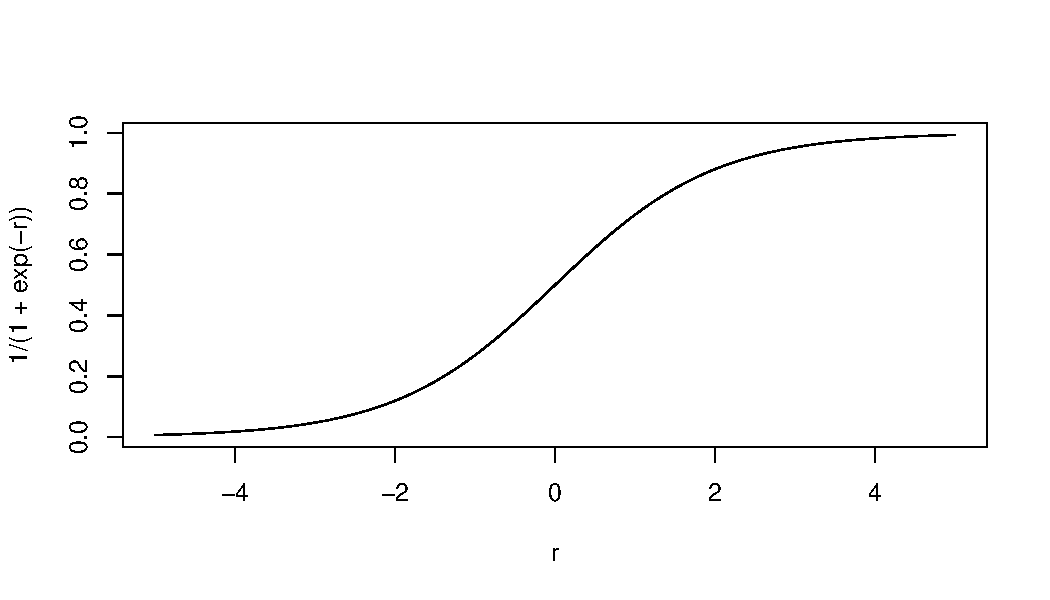
\includegraphics[width=\textwidth]{img/fig01.pdf}
\end{center}

\end{frame}

%%%%%%%%%%%%%%%%%%%%%%%%%%%%%%%%%%%%%%%%%%%%%%%%%%%
\begin{frame}[fragile] \frametitle{}

We could use other link functions $g$, the logit is simply
a popular choice given the theoretical connections to exponential
families.

\end{frame}

%%%%%%%%%%%%%%%%%%%%%%%%%%%%%%%%%%%%%%%%%%%%%%%%%%%
\begin{frame}[fragile] \frametitle{}

Assume instead that there exists a hidden variable $Z$ such that:
\begin{align*}
Z &= X\beta + \epsilon_i, \quad \epsilon_i \sim_{i.i.d.} \mathcal{N}(0, \sigma^2)
\end{align*}
And then:
\begin{align*}
y_i = \left\{ \begin{array}{c} 0, \, z_i < 0 \\ 1, \, z_i \geq 0 \end{array}  \right.
\end{align*}

\pause What link function would give us this model?

\end{frame}

%%%%%%%%%%%%%%%%%%%%%%%%%%%%%%%%%%%%%%%%%%%%%%%%%%%
\begin{frame}[fragile] \frametitle{}

\begin{center}
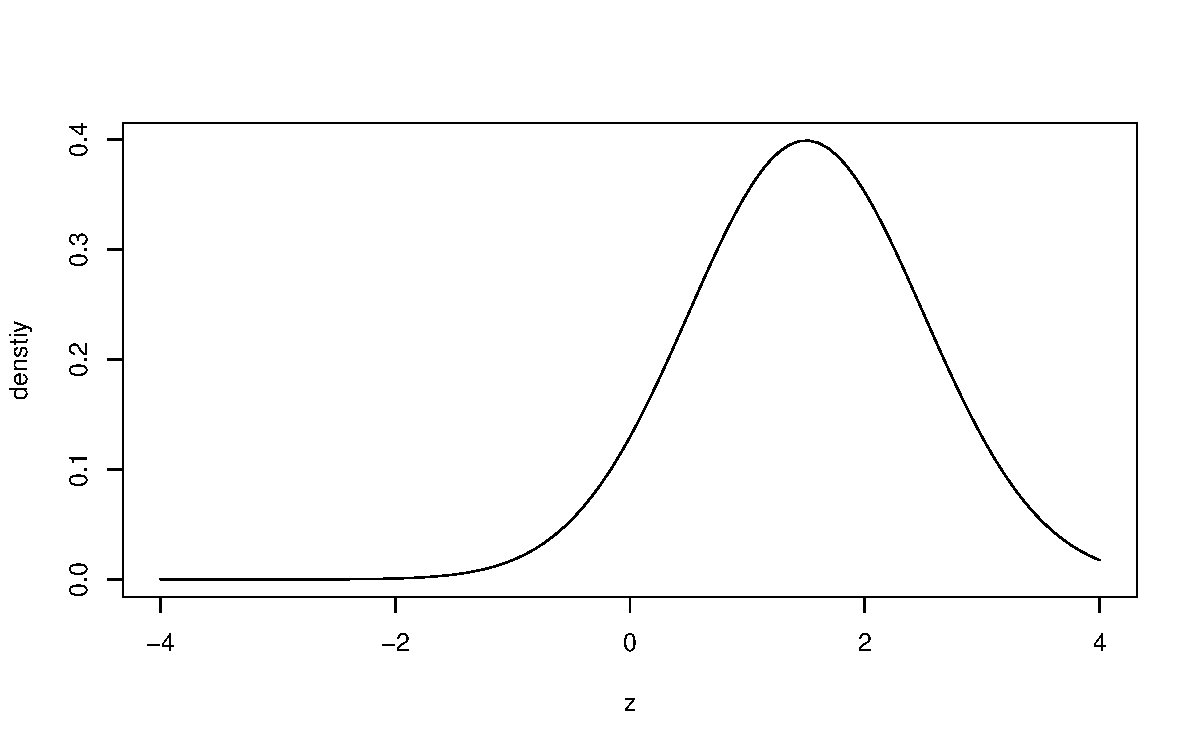
\includegraphics[width=\textwidth]{img/fig02a}
\end{center}

\end{frame}

%%%%%%%%%%%%%%%%%%%%%%%%%%%%%%%%%%%%%%%%%%%%%%%%%%%
\begin{frame}[fragile] \frametitle{}

\begin{center}
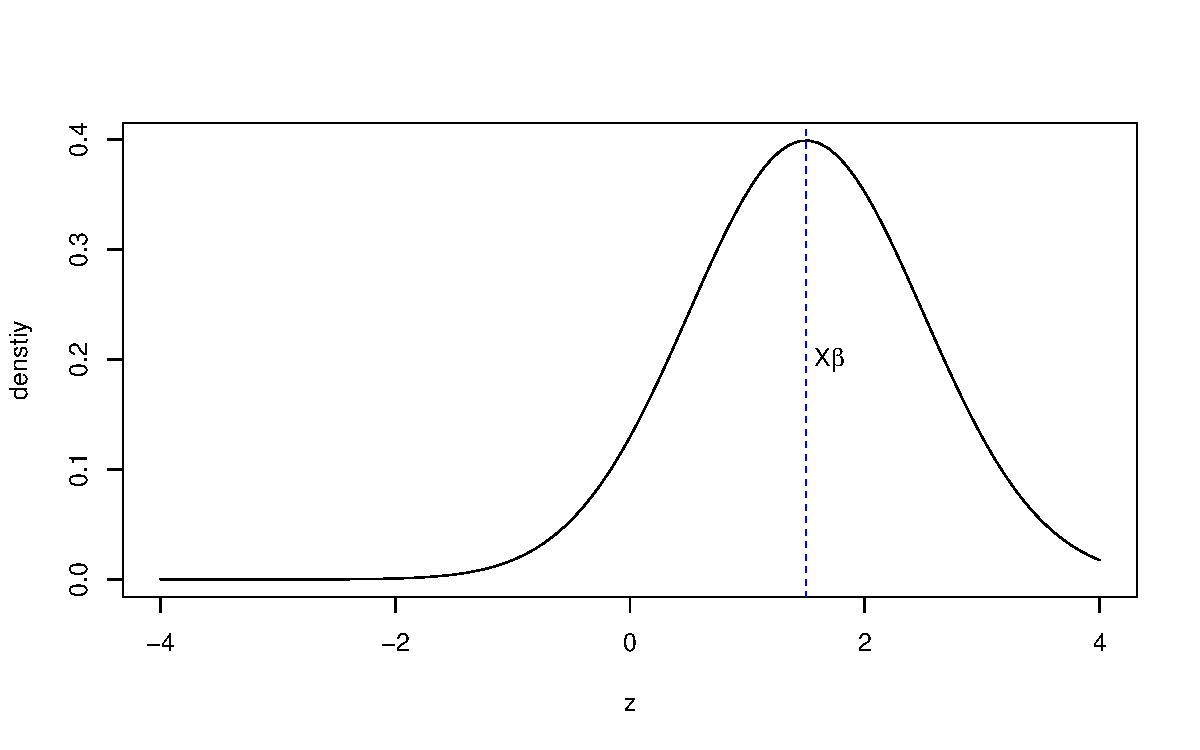
\includegraphics[width=\textwidth]{img/fig02b}
\end{center}

\end{frame}

%%%%%%%%%%%%%%%%%%%%%%%%%%%%%%%%%%%%%%%%%%%%%%%%%%%
\begin{frame}[fragile] \frametitle{}

\begin{center}
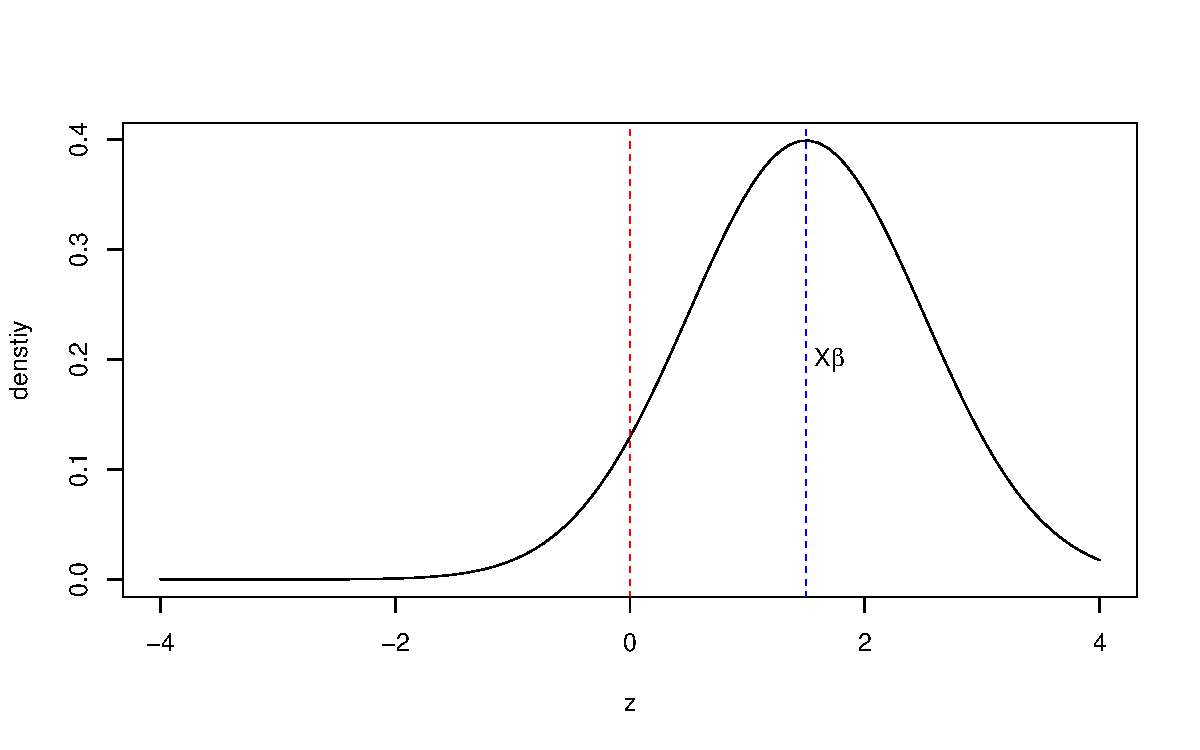
\includegraphics[width=\textwidth]{img/fig02c}
\end{center}

\end{frame}

%%%%%%%%%%%%%%%%%%%%%%%%%%%%%%%%%%%%%%%%%%%%%%%%%%%
\begin{frame}[fragile] \frametitle{}

\begin{center}
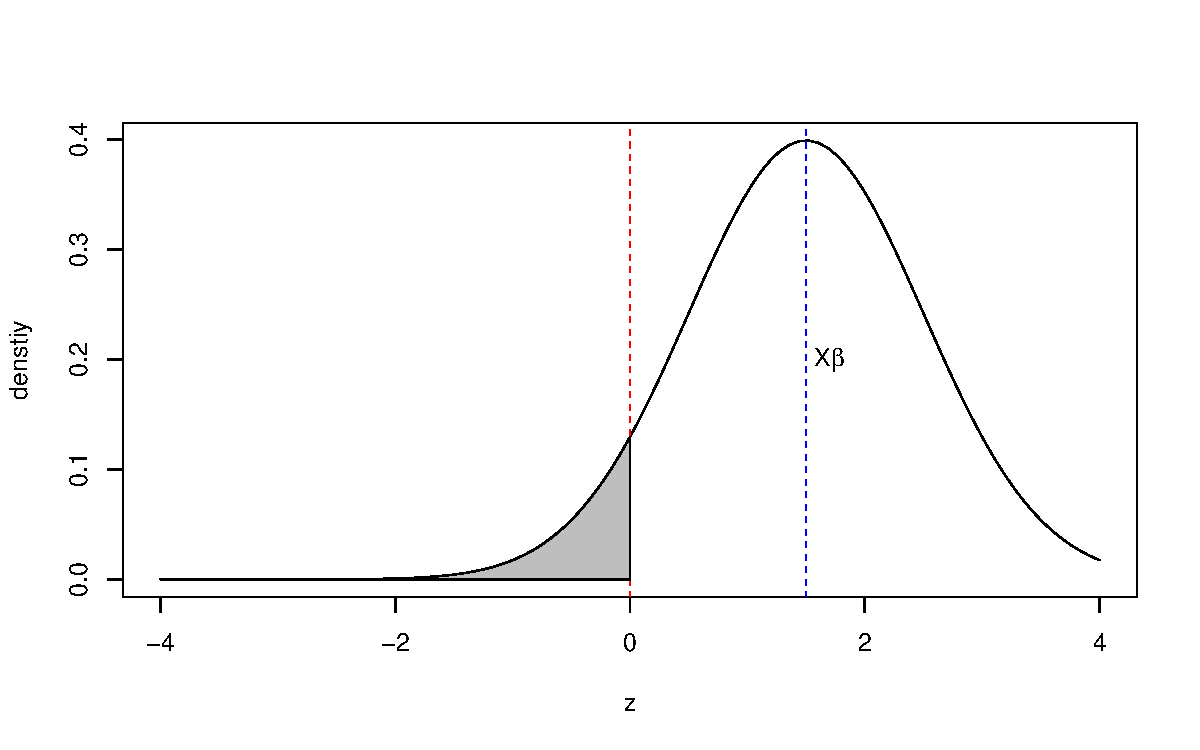
\includegraphics[width=\textwidth]{img/fig02d}
\end{center}

\end{frame}

%%%%%%%%%%%%%%%%%%%%%%%%%%%%%%%%%%%%%%%%%%%%%%%%%%%
\begin{frame}[fragile] \frametitle{}

\begin{center}
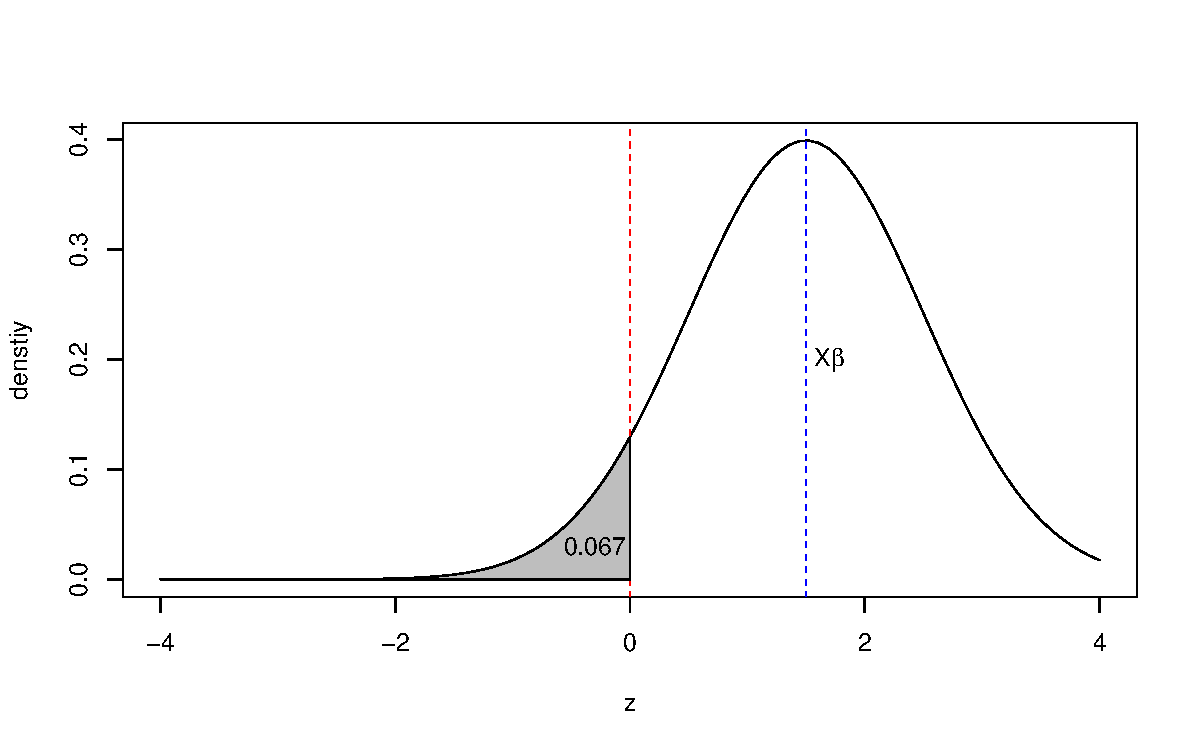
\includegraphics[width=\textwidth]{img/fig02e}
\end{center}

\end{frame}

%%%%%%%%%%%%%%%%%%%%%%%%%%%%%%%%%%%%%%%%%%%%%%%%%%%
\begin{frame}[fragile] \frametitle{}

So this model uses the inverse cdf of the standard normal
distribution:
\begin{align*}
\mathbb{E} (y | X) &= \Phi^{-1} (X\beta)
\end{align*}
Called the probit link. \pause Any other distribution with
support on the entire real line can be used.

\end{frame}

%%%%%%%%%%%%%%%%%%%%%%%%%%%%%%%%%%%%%%%%%%%%%%%%%%%
\begin{frame}[fragile] \frametitle{}

\begin{flushright}
{\color{yaleblue}\sc\fontsize{1cm}{0cm}\selectfont GLMs in R}
\end{flushright}

\end{frame}

% %%%%%%%%%%%%%%%%%%%%%%%%%%%%%%%%%%%%%%%%%%%%%%%%%%%
% \begin{frame}[fragile] \frametitle{}

% {\bf Deviance}

% Consider the likelihood for the classical linear regression
% model:
% \begin{align*}
% \mathcal{L}(y | x) &=  (2\pi\sigma^2)^{-n/2} \times
%     exp \left\{\frac{1}{2\sigma^2} || y - X\beta||_2^2 \right\}
% \end{align*}
% \pause If we take the log and remove the leading term that depends on
% only the $\sigma^2$ term we see that the log density is
% \begin{align*}
% l(y | x) &=  - \frac{1}{2\sigma^2} || y-X\beta ||_2^2
% \end{align*}
% \pause If we then multiply by $-2$, this yields the standardized sum
% of squares:
% \begin{align*}
% l(y | x) &=  || (y-X\beta) / \sigma ||_2^2
% \end{align*}

% \end{frame}


% %%%%%%%%%%%%%%%%%%%%%%%%%%%%%%%%%%%%%%%%%%%%%%%%%%%
% \begin{frame}[fragile] \frametitle{}

% {\bf Deviance}

% We know that this has a chi-square distribution
% \begin{align*}
% || (y-X\beta) / \sigma ||_2^2 \sim \chi^2_{n-p}
% \end{align*}

% \end{frame}


% %%%%%%%%%%%%%%%%%%%%%%%%%%%%%%%%%%%%%%%%%%%%%%%%%%%
% \begin{frame}[fragile] \frametitle{}

% {\bf Deviance, cont.}

% This notion also applies to generalized least squares. For logistic,
% regression we see that:
% \begin{align*}
% -2 \cdot l(y_i | x_i) = \left\{ \begin{array}{c} 2 \cdot \log\left(\frac{1}{1 - x_i^t \beta}\right), \, y_i = 0 \\ 2 \cdot \log\left(\frac{1}{x_i^t}\right), \, y_i = 1 \end{array}  \right.
% \end{align*}

% \end{frame}

\end{document}











